\section{Far-field sound localization using minimum-power SRP-PHAT}


\subsubsection{Using the redundant information from the microphone pairs}
A thing to note is that Eq. \ref{Eq:linearDep} is only true for no noise conditions. In case of low SNR, there is a potential to gain information by using the redundant microphone pairs. This is because if noise at all microphones is assumed to be uncorrelated, even though noise causes some microphone pairs to detect a source at a 'sourceless` location of the SRP search, certain microphone pairs will have a lower magnitude at that location. So in case of a SRP-PHAT, the sum of all microphone pairs will be higher at the real source location, and at other locations, the sum due to the noise will be suppressed. Fig. \ref{fig:4mic1srcRedun} shows the effect of using all microphone pairs for noisy conditions. Note that the dynamic range in the figure has been lowered to highlight the differences. It can be seen that using all the microphone pairs adds to the overall noise as more pairs can now contribute to the SRP sum, however, ideally the peak of the true source would also be higher, due to more pairs providing power at the source location. 
\begin{figure}[H]
\begin{subfigure}[b]{0.96\textwidth}
    \centering
    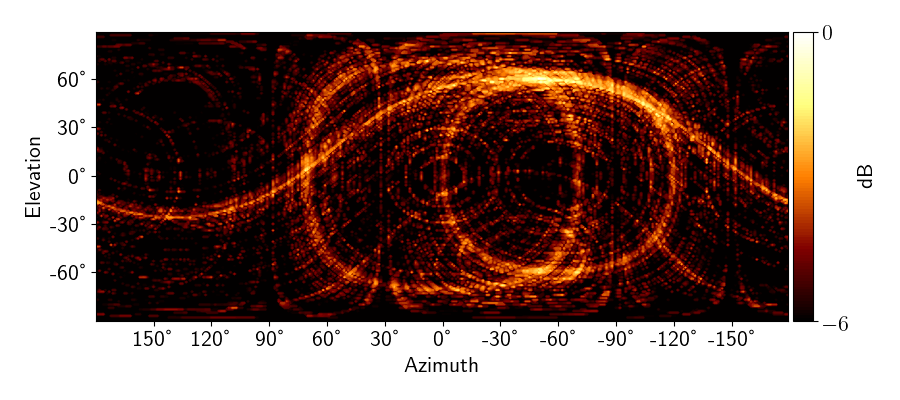
\includegraphics[width=0.8\textwidth]{Figures/Ind4mic1srcResNeg10LowDyn.png}
\end{subfigure}
\vskip \baselineskip
\begin{subfigure}[b]{0.96\textwidth}
    \centering
    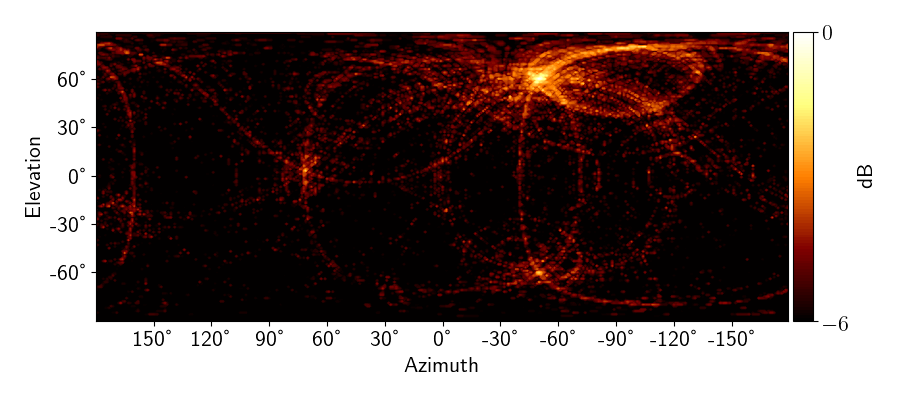
\includegraphics[width=0.8\textwidth]{Figures/Dep4mic1srcResNeg10LowDyn.png}
\end{subfigure}
\caption{Figures depict from SRP-PHAT localization results with SNR = -10dB, for independent microphone pairs (top), and for all  microphone pairs (bottom)}
\label{fig:4mic1srcRedun}
\end{figure}






